%\pdfoutput=1 %for arXiv submission
%\documentclass[iop,apj]{emulateapj}
\documentclass[twocolumn]{aastex63}
\usepackage{hyperref}
\usepackage{amsmath,amstext}
\usepackage[T1]{fontenc}
%\usepackage{apjfonts} 
\usepackage{graphicx}
\usepackage[figure,figure*]{hypcap}
%\usepackage[fleqn]{amsmath}
\usepackage{multirow}
\usepackage{comment}
\usepackage{nicefrac}

\renewcommand*{\sectionautorefname}{Section} %for \autoref
\renewcommand*{\subsectionautorefname}{Section} %for \autoref

\def\lbol{${L}_{\rm bol}$}
\def\ledd{${L}_{\rm Edd}$}
\def\lsun{${L}_{\odot}$}
\def\sun{$_{\odot}$}
\def\lx{${L}_{\rm X}$}
\def\fx{${f}_{\rm X}$}
\def\f28{${f}_{2-8{\rm keV}}$}
\def\fr{${f}_R$}
\def\fo{f$_{opt}$}
\def\fxfr{${f}_X$/${f}_R$}
\def\fratio{${f}_X$/${f}_R$} 
\def\fxfopt{${f}_X$/${f}_{opt}$}
\def\fxfV{${f}_X$/${f}_V$}
\def\nh{N$_{\rm H}$}
\def\rc{r$_c$}
\def\mass{${\cal M}$}
\def\msun{${\cal M}_{\odot}$}
\def\mearth{${\cal M}_{\oplus}$}
\def\sun{$_{\odot}$}
\def\mdot{$\dot{\cal M}$}

\def\ergs{erg s$^{-1}$}
\def\ergscm2{erg s$^{-1}$ cm$^{-2}$}
\def\yr-1{yr$^{-1}$}
\def\kms{km s$^{-1}$}
\def\persec{\,\hbox{s}^{-1}}
\def\percc{\,\hbox{cm}^{-3}}
\def\persqcm{\,\hbox{cm}^{-2}}
\def\mic{\,\mu \hbox{m}}

\def\eg{{\it e.g.}}
\def\et{{\it et al.}}
\def\ie{{\it i.e.}}
\def\cf{{\it cf.}}

\def\a{$\&$}
\def\x{$\times$}
\def\about{$\sim$}
\def\simlt{\buildrel{<}\over \sim}
\def\simgt{\buildrel{>}\over \sim}
\def\simeq{\sim \over $=$}
\def\simgreat{\buildrel{>}\over \sim}
\def\simlt{$\la$}
\def\simgt{$\ga$}
\def\half{${\textstyle{1\over2}}$}
\def\thalf{{\textstyle{ 3\over 2}}}
\def\subr #1{_{{\rm #1}}}
\def\w{$\omega$}
\def\sig{$\sigma$}

\def\deg{$^{\rm o}$}
%\def\asec{$''$} 
\def\asec{\ifmmode^{\prime\prime}\else$^{\prime\prime}$\fi}
\def\amin{$'$}
\def\spt{$\buildrel{\prime\prime}\over .$}
\def\secspt{$\buildrel{\prime\prime}\over .$}
\def\minspt{$\buildrel{\prime}\over .$}
\def\magspt{$\buildrel{\rm m}\over .$}

%\def\Chandra{{\it Chandra}}
%\def\XMM{XMM {\it Newton}}
%\def\Rosat{{\it Rosat}}
%\def\Einstein{{\it Einstein}}
%\def\HST{{\it HST}}
%\def\Swift{{\it Swift}}
%\def\Nustar{{\it NuSTAR}}

\hypersetup{linkcolor=magenta}

\submitjournal{ApJ}
\received{December 31, 2020}

\shorttitle{$r$-process abundances and kilonovae} 
\shortauthors{Vieira {\it et al.}}

\begin{document}

\title{Spectral $r$-Process Abundance Retrieval for Kilonovae: \textsc{SPARK}}

\correspondingauthor{Nicholas~Vieira}
\email{nicholas.vieira@mail.mcgill.ca}

\author[0000-0001-7815-7604]{Nicholas~Vieira}
\affil{McGill Space Institute and Department of Physics, McGill University, 3600 rue University, Montreal, Quebec, H3A 2T8, Canada}

\author[0000-0001-8665-5523]{John~J.~Ruan}
\affil{Physics and Astronomy Department, Bishop's University, 2600 College St, Sherbrooke, Quebec, J1M 1Z7, Canada}
%\affil{McGill Space Institute and Department of Physics, McGill University, 3600 rue University, Montreal, Quebec, H3A 2T8, Canada}

\author[0000-0001-6803-2138]{Daryl Haggard}
\affil{McGill Space Institute and Department of Physics, McGill University, 3600 rue University, Montreal, Quebec, H3A 2T8, Canada}
\affil{CIFAR Azrieli Global Scholar, Gravity \& the Extreme Universe Program, Canadian Institute for Advanced Research, 661 University Avenue,
Suite 505, Toronto, Ontario, M5G 1M1, Canada}

%\author[0000-0001-7081-0082]{Maria~R.~Drout}
%\affil{Department of Astronomy and Astrophysics, University of Toronto, 50 St. George St., Toronto, Ontario, M5S 3H4, Canada}

\begin{abstract}
\end{abstract}
\keywords{TBD}

% ====================================================

%%% === SECTION 1 === %%%
%% INTRODUCTION %%
\section{Introduction}\label{sec:intro}
The mergers of neutron stars (NSMs) or a black hole (BH) and neutron star (NS-BH) have long been suspected as a site of astrophysical rapid neutron capture, or the \textit{r}-process (\citealt{lattimer74, eichler89, freiburghaus99}). A major goal of astronuclear physics is to determine if these events can robustly produce the "universal" \textit{r}-process abundances observed in the Sun, galactic halo stars, and ultra-faint dwarf galaxies (\citealt{ji16, cote18} \textbf{+ much more}). Various lines of evidence ranging from hierarchical merger simulations of dwarf galaxies to form the Milky Way (\citealt{ishimaru15}) to the abundances of the actinides in meteorites (\citealt{bartos19}) have suggested that these events may indeed be the dominant source of the \textit{r}-process elements in the universe. However, there is still much debate, and certain classes of core-collapse supernovae (CCSNe, or "collapsars") may also contribute substantially to the universal \textit{r}-process or in fact dominate over NSMs (\citealt{siegel19}).

The landmark multi-messenger event GW170817, which was detected both in gravitational waves (GWs) and electromagnetic (EM) waves, offered the first direct test of the ability of NSMs to robustly synthesize the r-process elements. The abundances of the elements in the universal \textit{r}-process are characterized by three broad peaks in the vicinity of atomic mass $A\sim80$ ($Z\sim35$, Br), $\sim130$ ($Z\sim52$, Te) and $\sim195$ ($Z\sim79$, Au), in order of decreasing abundance. A sub-peak around $A\sim150$ in the vicinity of the lanthanides ($Z=57-70$, La$-$Yb) is also observed. In this context, "robust" \textit{r}-process nucleosynthesis involves the synthesis of all three of these peaks. Optical/infra-red (IR) photometric (\citealt{andreoni17, arcavi17, coulter17, diaz17, drout17, evans17, hu17, kasliwal17, lipunov17, shappee17, tanvir17, troja17, utsumi17, valenti17}) and spectroscopic (\citealt{kasen17, pian17, smartt17, cote18} \textbf{+ much more}) observations of the EM counterpart of GW170817, named AT2017gfo, broadly confirmed the presence of a transient kilonova (KN) powered by the radioactive decay of freshly-synthesized \textit{r}-process elements. However, whether the quantity of lanthanides (and heavier elements) matches that expected by the universal \textit{r}-process is unclear. Indeed, \cite{ji19} reviewed the lanthanide mass fraction $X_{\mathrm{lan}}$ inferred across the literature and broadly found that the lanthanides were under-produced in AT2017gfo relative to the \textit{r}-process abundances present in galactic halo stars. They concluded that some fraction of future KNe would need to be significantly 'redder' for NSMs to be the dominant source of \textit{r}-process elements in the Universe. 

\begin{itemize}
    \item Discussion on the origin of the $r$-process. Long-standing possibility that NSMs are one of the sites of the astrophysical r-process (\citealt{lattimer74, eichler89, freiburghaus99}). 
    
    \item Possibility of NSMs further being the dominant source of the $r$-process in the MW, according to various lines of evidence, e.g. simulations of the hierarchical mergers of dwarf galaxies (\citealt{ishimaru15}) and actinide abundances in meteorites (\citealt{bartos19}).
    
    
    \item Possibility of collapsars being the dominant site instead (\citealt{siegel19}).
    
    
    \item Observations of galactic halo stars, $r$-process enriched stars, faint dwarf galaxies... (\citealt{ji16, cote18} \textbf{+ much more}).
    
    
    \item Various conclusions drawn from GW170817 (\citealt{kasen17, pian17, smartt17, cote18, rosswog18} \textbf{+ much more}). Observed inconsistency between the lanthanide fraction of GW170817 in the literature and metal-rich galactic halo stars (\citealt{ji19}).

    
    \item Strontium II in X-shooter spectra of GW170817 (\citealt{watson19}).
\end{itemize}

%%% === SECTION 2 === %%%
%% METHODS %%
\section{Methods}\label{sec:methods}

\subsection{Atomic Structure Calculations}\label{ssc:atomic}
\begin{itemize}
    \item We use \texttt{AUTOSTRUCTURE} (\citealt{badnell16}).
    
    \item Optimization scheme based on that of \cite{kasen13}.
    
    \item Discussion of previous incomplete attempts at atomic structure calculations (\citealt{kasen13, tanaka18}).
    
    \item Carrying out systematic atomic structure calculations. Electron configurations are those of \cite{tanaka20} (first systematic atomic structure calculations) except where stated otherwise.
    
    \item National Institute of Standards and Technology (NIST) used for reference (\citealt{kramida19}).
    
    \item For elements from $Z=26$ to $88$, find a total of approximately $2.2\times10^9$ lines.
    
    \item Use of the Kurucz line list (\citealt{kurucz95}) for elements with $Z\leqslant25$.
    
\end{itemize}

\subsection{Elemental Abundances}
\begin{itemize}
    \item Solar $r$-process (\citealt{sneden08}).
    
    \item Variety of abundance patterns depending on the component in question. Disk wind abundances (\citealt{wu16}).
    
    \item Abundances from \cite{wanajo14}? \cite{wanajo18}?
    
    \item Importance of certain elements, e.g. neodymium (Nd) and possibly uranium (U) (\citealt{kasen17, even19} \textbf{+ much more}).
    
    \item Impact of uncertainties in nuclear models (specifically, the nuclear masses, fission process and fragment distributions, neutron capture rates, $\beta$-decay rates) on abundances and especially on those of the heaviest elements (\citealt{eichler15, barnes16, cote18} \textbf{+ much more, e.g. Mumpower papers}).
\end{itemize}

\subsection{Radiative Transfer with \textsc{TARDIS}}\label{ssc:TARDIS}
\begin{itemize}

    \item We use \texttt{TARDIS} (Temperature And Radiative Diffusion In Supernovae), a Monte Carlo radiative transfer tool (\citealt{kerzendorf14}).
    
    \item When constructing atomic data files, for computational feasibility, we use only the strongest lines from our line list. We use lines with $\log_{10}(g \cdot f) \geqslant -3$, where $g \cdot f$ is the product of the statistical weight $g$ of an energy level and oscillator strength $f$ of a transition. $g \cdot f$ is sometimes called the 'symmetric oscillator strength' because $|g\cdot f| \equiv |g_1 \cdot f_{12}| = |g_2 \cdot f_{21}|$, where $f_{21}$ and $f_{12}$ are the oscillator strengths for absorption and emission, respectively. This cut results in a reduction from $2.2 \times 10^9$ lines to $1.6 \times 10^8$ lines, i.e., a 92.8\% decrease.
\end{itemize}

\subsection{Parameter Estimation with \textsc{approxposterior}}\label{ssc:approxposterior}
\begin{itemize}
    \item We use \texttt{approxposterior} (\citealt{fleming18}), which makes use of the Bayesian Active Posterior Estimation (BAPE) algorithm of \cite{kandasamy17} and the methods of \cite{wang18} for Bayesian inference involving expensive likelihood functions with adaptive Gaussian processes.
\end{itemize}

\subsection{GW170817}\label{ssc:GW170817}
\begin{itemize}
    \item VLT/X-shooter spectra (\citealt{pian17, smartt17}) acquired through WISeREP (\citealt{yaron12}).
\end{itemize}

%%% === SECTION 3 === %%%
%% WHO KNOWS %%
\section{Results}\label{sec:results}


%%% === SECTION 4 === %%%
%% DISCUSSION %%
\section{Discussion}\label{sec:disco}
\begin{itemize}
    \item Discussion on viewing angle dependence and imprint on LCs and spectra? (\citealt{darbha20, korobkin20}). Mention importance of pinning down the viewing angle with sufficient accuracy to avoid systematic bias in measurement of $H_0$? (\citealt{chen20}).
    
    \item Discussion on ability of late-time KNe, when isotopes of just a few elements e.g. californium (${}^{254}$Cf) dominate, to provide special insights? (\citealt{villar18, wanajo18, zhu18, kasliwal19, wu19} \textbf{+ much more}). 
\end{itemize}

%%% === SECTION 5 === %%%
%% CONCLUSIONS %%
\section{Conclusions}\label{sec:conclusions}

%%% === ACKNOWLEDGEMENTS === %%%
\acknowledgments
We thank Dr. N. Badnell for many useful discussions and assistance in operating \texttt{AUTOSTRUCTURE}. We thank Dr. M. Tanaka and collaborators for graciously sharing their line list. N.V. acknowledges funding from the Natural Sciences and Engineering Research Council of Canada (NSERC), Fonds de recherche du Qu\'ebec - Nature et Technologies (FRQNT), and the Bob Wares Science Innovation Prospectors Fund. J.J.R.\ and D.H.\ acknowledge support from a NSERC Discovery Grant, a  FRQNT Nouveaux Chercheurs Grant, and support from the Canadian Institute for Advanced Research (CIFAR).  J.J.R.\ acknowledges funding from the McGill Trottier Chair in Astrophysics and Cosmology, the McGill Space Institute, and the Dan David Foundation.

This work made extensive use of the \href{https://docs.computecanada.ca/wiki/Cedar}{\texttt{Cedar}} cluster of \href{https://www.computecanada.ca/home/}{Compute Canada} at Simon Fraser University, with regional partner \href{https://www.westgrid.ca/}{WestGrid}. This research made use of \texttt{TARDIS}, a community-developed software package for spectral synthesis in supernovae (\citealt{kerzendorf14}). The development of \texttt{TARDIS} received support from the Google Summer of Code initiative and from the European Space Agency (ESA)'s Summer of Code in Space program. \texttt{TARDIS} makes extensive use of \texttt{astropy} and \texttt{PyNE}. 
\newline
%%% === SOFTWARE === %%%
\software{
\href{https://dflemin3.github.io/approxposterior/index.html}{\texttt{approxposterior}}: \cite{fleming18};
\href{https://docs.astropy.org/en/stable/}{\texttt{astropy}}: \cite{astropy18};
\href{http://amdpp.phys.strath.ac.uk/autos/}{\texttt{AUTOSTRUCTURE}} v27: \cite{badnell16};
\href{https://corner.readthedocs.io/en/latest/index.html}{\texttt{corner}}: \cite{foreman-mackey16};
\href{https://emcee.readthedocs.io/en/stable/}{\texttt{emcee}}: \cite{foreman-mackey13};
\href{https://george.readthedocs.io/en/latest/}{\texttt{george}}: \cite{ambikasaran15};
\href{https://tardis-sn.github.io/tardis/index.html}{\texttt{TARDIS}}: \citealt{kerzendorf14}
} 

\clearpage
%%% === BILBIOGRAPHY === %%%
\bibliographystyle{apj}
\begin{thebibliography}{}

\bibitem[Abbott et al.(2017a)]{abbottLIGO17a} Abbott, B.~P., Abbott, R., Abbott, T.~D., et al.\ 2017a, \aj, 848, L12

%\bibitem[Abbott et al.(2017b)]{abbottLIGO17b} Abbott, B.~P., Abbott, R., Abbott, T.~D., et al.\ 2017b, \apjl, 848, L13

%\bibitem[Abbott et al.(2018)]{abbottLIGO18} Abbott, B.~P., Abbott, R., Abbott, T.~D., et al.\ 2018, Living Reviews in Relativity, 21, 3

%\bibitem[Abbott et al.(2018)]{abbott18} Abbott, T.~M.~C., Abdalla, F.~B., Allam, S., et al.\ 2018, \apjs, 239, 18

\bibitem[Ambikasaran et al.(2015)]{ambikasaran15} Ambikasaran, S., Foreman-Mackey, D., Greengard, L., et al.\ 2015, IEEE Transactions on Pattern Analysis and Machine Intelligence, 38, 252

\bibitem[Andreoni et al.(2017)]{andreoni17} Andreoni, I., Ackley, K., Cooke, J., et al.\ 2017, \pasa, 34, e069
%%%%% GW170817 observations paper

\bibitem[Arcavi et al.(2017)]{arcavi17} Arcavi, I., Hosseinzadeh, G., Howell, D.~A., et al.\ 2017, \nat, 551, 64
%%%%% GW170817 observations paper

\bibitem[Arnett(1982)]{arnett82} Arnett, W.~D.\ 1982, \apj, 253, 785

\bibitem[Astropy Collaboration et al.(2018)]{astropy18} Astropy Collaboration, Price-Whelan, A.~M., Sip{\H{o}}cz, B.~M., et al.\ 2018, \aj, 156, 123

\bibitem[Badnell(2016)]{badnell16} Badnell, N.~R.\ 2016, AUTOSTRUCTURE: General program for calculation of atomic and ionic properties, ascl:1612.014

%\bibitem[Barnes \& Kasen(2013)]{barnes13} Barnes, J., Kasen, D.\ 2013, \aj, 775, 18

\bibitem[Barnes et al.(2016)]{barnes16} Barnes, J., Kasen, D., Wu, M., Mart\'{i}nez-Pinedo, G.\ 2016, \aj,  829, 110

%\bibitem[Barstow \& Heng(2020)]{barstow20} Barstow, J.~K., \& Heng, K.\ 2020, arXiv e-prints, arXiv:2003.14311


\bibitem[Bartos \& Marka(2019)]{bartos19} Bartos, I. \& Marka, S.\ 2019, \nat, 569, 85

%\bibitem[Bethe \& Brown(1998)]{bethe98} Bethe, H.~A., \& Brown, G.~E.\ 1998, \apj, 506, 780


%\bibitem[Chatzopoulos et al.(2012)]{chatzopoulos12} Chatzopoulos, E., Wheeler, J.~C., Vinko, J.\ 2012, \aj, 746, 121 

\bibitem[Chen(2020)]{chen20} Chen, H.-Y.\ 2020, arXiv e-prints, arXiv:2006.02779


%\bibitem[Christie et al.(2019)]{christie19} Christie, I.~M., Lalakos, A., Tchekhovskoy, A., et al.\ 2019, \mnras, 490, 4811

\bibitem[C{\^o}t{\'e} et al.(2018)]{cote18} C{\^o}t{\'e}, B., Fryer, C.~L., Belczynski, K., et al.\ 2018, \apj, 855, 99

\bibitem[Coulter et al.(2017)]{coulter17} Coulter, D.~A., Foley, R.~J., Kilpatrick, C.~D., et al.\ 2017, Science, 358, 1556
%%%%% GW170817 observations paper

\bibitem[Darbha \& Kasen(2020)]{darbha20} Darbha, S., \& Kasen, D.\ 2020, arXiv e-prints, arXiv:2002.00299

\bibitem[D{\'\i}az et al.(2017)]{diaz17} D{\'\i}az, M.~C., Macri, L.~M., Garcia Lambas, D., et al.\ 2017, \apjl, 848, L29
%%%%% GW170817 observations paper

\bibitem[Drout et al.(2017)]{drout17} Drout, M.~R., Piro, A.~L., Shappee, B.~J., et al.\ 2017, Science, 358, 6370, 1570-1574
%%%%% GW170817 observations paper

\bibitem[Eichler et al.(1989)]{eichler89} Eichler, D., Livio, M., Piran, T., et al.\ 1989, \nat, 340, 126

\bibitem[Eichler et al.(2015)]{eichler15} Eichler, M., Arcones, A., Kelic, A., et al.\ 2015, \apj, 808, 30

%\bibitem[Etienne et al.(2009)]{etienne09} Etienne, Z.~B., Liu, Y.~T., Shapiro, S.~L.\ 2009, \prd, 79, 044024

\bibitem[Evans et al.(2017)]{evans17} Evans, P.~A., Cenko, S.~B., Kennea, J.~A., et al.\ 2017, Science, 358, 1565
%%%%% GW170817 observations paper

\bibitem[Even et al.(2019)]{even19} Even, W., Korobkin, O., Fryer, C.~L., et al.\ 2019, arXiv e-prints, arXiv:1904.13298

%\bibitem[Fern{\'a}ndez \& Metzger(2013)]{fernandez13} Fern{\'a}ndez, R., \& Metzger, B.~D.\ 2013, \mnras, 435, 502

%\bibitem[Fern{\'a}ndez et al.(2017)]{fernandez17} Fern{\'a}ndez, R., Foucart, F., Kasen, D., et al.\ 2017, Classical and Quantum Gravity, 34, 154001

%\bibitem[Fern{\'a}ndez et al.(2019)]{fernandez19} Fern{\'a}ndez, R., Tchekhovskoy, A., Quataert, E., et al.\ 2019, \mnras, 482, 3373

\bibitem[Fleming \& VanderPlas(2018)]{fleming18} Fleming, D.~P., \& VanderPlas, J.\ 2018, The Journal of Open Source Software, 3, 781

\bibitem[Fleming et al.(2020)]{fleming20} Fleming, D.~P., Barnes, R., Luger, R., et al.\ 2020, \apj, 891, 155

\bibitem[Foreman-Mackey et al.(2013)]{foreman-mackey13} Foreman-Mackey, D., Hogg, D.~W., Lang, D., et al.\ 2013, \pasp, 125, 306

\bibitem[Foreman-Mackey(2016)]{foreman-mackey16} Foreman-Mackey, D.\ 2016, The Journal of Open Source Software, 1, 24

%\bibitem[Foucart et al.(2014)]{foucart14} Foucart, F., Deaton, M.~B., Duez, M.~D., et al.\ 2014, \prd, 90, 024026

%\bibitem[Foucart et al.(2018)]{foucart18} Foucart, F., Hinderer, T., \& Nissanke, S.\ 2018, \prd, 98, 081501

%\bibitem[Foucart et al.(2019)]{foucart19} Foucart, F., Duez, M.~D., Kidder, L.~E., et al.\ 2019, \prd, 99, 103025

\bibitem[Freiburghaus et al.(1999)]{freiburghaus99} Freiburghaus, C., Rosswog, S., \& Thielemann, F.-K.\ 1999, \apjl, 525, L121

\bibitem[Hu et al.(2017)]{hu17} Hu, L., Wu, X., Andreoni, I., et al.\ 2017, Science Bulletin, 62, 1433
%%%%% GW170817 observations paper

\bibitem[Ishimaru et al.(2015)]{ishimaru15} Ishimaru, Y., Wanajo, S., \& Prantzos, N.\ 2015, \apjl, 804, L35

\bibitem[Ji et al.(2016)]{ji16} Ji, A.~P., Frebel, A., Chiti, A., et al.\ 2016, \nat, 531, 610

\bibitem[Ji et al.(2019)]{ji19} Ji, A.~P., Drout, M.~R., \& Hansen, T.~T.\ 2019, \apj, 882, 40

%\bibitem[Just et al.(2015)]{just15} Just, O., Bauswein, A., Ardevol Pulpillo, R., et al.\ 2015, \mnras, 448, 541

\bibitem[Kandasamy et al.(2017)]{kandasamy17} Kandasamy, K., Schneider, J., P{\'o}czos, B.\ 2017, Artificial Intelligence, 243

\bibitem[Kasen et al.(2013)]{kasen13}Kasen, D., Badnell, N.~R., Barnes, J., \ 2013, \aj, 774, 25

\bibitem[Kasen et al.(2017)]{kasen17} Kasen, D., Metzger, B., Barnes, J., et al.\ 2017, \nat, 551, 80

%\bibitem[Kasen \& Barnes(2019)]{kasen19} Kasen, D., \& Barnes, J.\ 2019, \apj, 876, 128

\bibitem[Kasliwal et al.(2017)]{kasliwal17} Kasliwal, M.~M., Nakar, E., Singer, L.~P., et al.\ 2017, Science, 358, 1559
%%%%% GW170817 observations paper

\bibitem[Kasliwal et al.(2019)]{kasliwal19} Kasliwal, M.~M., Kasen, D., Lau, R.~M., et al.\ 2019, \mnras, L14

%\bibitem[Kawaguchi et al.(2015)]{kawaguchi15} Kawaguchi, K., Kyutoku, K., Nakano, H., et al.\ 2015, \prd, 92, 024014

%\bibitem[Kawaguchi et al.(2016)]{kawaguchi16} Kawaguchi, K., Kyutoku, K., Shibata, M., Tanaka, M.\ 2016, \aj, 825, 52

\bibitem[Kerzendorf \& Sim(2014)]{kerzendorf14} Kerzendorf, W.~E., \& Sim, S.~A.\ 2014, \mnras, 440, 387

\bibitem[Khatami \& Kasen(2019)]{khatami19} Khatami, D.~K., \& Kasen, D.~N.\ 2019, \apj, 878, 56

\bibitem[Korobkin et al.(2012)]{korobkin12} Korobkin, O., Rosswog, S., Arcones, A., Winteler, C., et al.\ 2012, \mnras, 426, 3, 1940-1949

\bibitem[Korobkin et al.(2020)]{korobkin20} Korobkin, O., Wollaeger, R., Fryer, C., et al.\ 2020, arXiv e-prints, arXiv:2004.00102


\bibitem[Kramida et al.(2019)]{kramida19} Kramida, A., Ralchenko, Y., Reader, J., and {NIST ASD Team} \ 2019, NIST Atomic Spectra Database (ver 5.7.1), National Institute of Standards and Technology

\bibitem[Kurucz \& Bell(1995)]{kurucz95} Kurucz, R., \& Bell, B.\ 1995, Atomic Line Data (R.L. Kurucz and B. Bell) Kurucz CD-ROM No. 23. Cambridge, 23

%\bibitem[Kyutoku et al.(2015)]{kyutoku15} Kyutoku, K., Ioka, K., Okawa, H., et al.\ 2015, \prd, 92, 044028

%\bibitem[Kyutoku et al.(2018)]{kyutoku18} Kyutoku, K., Kiuchi, K., Sekiguchi, Y., et al.\ 2018, \prd, 97, 023009

\bibitem[Lattimer \& Schramm(1974)]{lattimer74} Lattimer, J.~M., \& Schramm, D.~N.\ 1974, \apjl, 192, L145

%\bibitem[Li \& Paczy{\'n}ski(1998)]{li98} Li, L.-X., \& Paczy{\'n}ski, B.\ 1998, \apjl, 507, L59

\bibitem[Lippuner \& Roberts(2015)]{lippuner15} Lippuner, J. \& Roberts, L.~F.\ 2015, \apj, 815, 82

%\bibitem[Lippuner et al.(2017)]{lippuner17} Lippuner, J., Fern\'{a}ndez, R., Roberts, L.~F., et al.\ 2017, \mnras, 472, 1, 904-918

\bibitem[Lipunov et al.(2017)]{lipunov17} Lipunov, V.~M., Gorbovskoy, E., Kornilov, V.~G., et al.\ 2017, \apjl, 850, L1
%%%%%% GW170817 observations paper

%\bibitem[Lovelace et al.(2013)]{lovelace13} Lovelace, G., Duez, M.~D., Foucart, F., et al.\ 2013, Class. Quant. Grav., 30, 13

%\bibitem[Metzger et al.(2008)]{metzger08} Metzger, B.~D., Piro, A.~L., \& Quataert, E.\ 2008, \mnras, 390, 781

\bibitem[Metzger et al.(2010)]{metzger10} Metzger, B.~D., Mart{\'i}nez-Pinedo, G., Darbha, S., et al.\ 2010, \mnras, 406, 4, 2650-2662

%\bibitem[Metzger \& Fern{\'a}ndez(2014)]{metzger14} Metzger, B.~D., \& Fern{\'a}ndez, R.\ 2014, \mnras, 441, 3444

\bibitem[Metzger(2019)]{metzger19} Metzger, B.~D.\ 2019, Living Rev Relativ, 23, 1
%%%%%% tome on KNe

\bibitem[Pian et al.(2017)]{pian17} Pian, E., D'Avanzo, P., Benetti, S., et al.\ 2017, \nat, 551, 67
%%%%%% GW170817 spectra paper

%\bibitem[Planck Collaboration et al.(2016)]{planck16} Planck Collaboration, Ade, P.~A.~R., Aghanim, N., et al.\ 2016, \aap, 594, A13
%%%%% Lambda-CDM cosmology

%\bibitem[Pozanenko et al.(2018)]{pozanenko18} Pozanenko, A.~S., Barkov, M.~V., Minaev, P.~Y., et al.\ 2018, \apjl, 852, L30
%%%%% GW170817 observations paper

%\bibitem[Rosswog(2005)]{rosswog05} Rosswog, S.\ 2005, \aj, 634, 1202

\bibitem[Rosswog et al.(2018)]{rosswog18} Rosswog, S., Sollerman, J., Feindt, U., et al.\ 2018, \aap, 615, A132

%\bibitem[Ruiz et al.(2018)]{ruiz18} Ruiz, M., Shapiro, S.~L., \& Tsokaros, A.\ 2018, \prd, 98, 123017

%\bibitem[Sagu{\'e}s Carracedo et al.(2020)]{carracedo20} Sagu{\'e}s Carracedo, A., Bulla, M., Feindt, U., et al.\ 2020, arXiv e-prints, arXiv:2004.06137

%\bibitem[Schlafly \& Finkbeiner(2011)]{schlafly11} Schlafly, E.~F., \& Finkbeiner, D.~P.\ 2011, \apj, 737, 103
%%%%% computing extinctions

%\bibitem[Scolnic et al.(2018)]{scolnic18} Scolnic, D., Kessler, R., Brout, D., et al.\ 2018, \apjl, 852, L3

%\bibitem[Setzer et al.(2019)]{setzer19} Setzer, C.~N., Biswas, R., Peiris, H.~V., et al.\ 2019, \mnras, 485, 4260

\bibitem[Shappee et al.(2017)]{shappee17} Shappee, B.~J., Simon, J.~D., Drout, M.~R., et al.\ 2017, Science, 358, 1574
%%%%% GW170817 observations paper

%\bibitem[Shibata \& Taniguchi(2008)]{shibata08} Shibata M., \& Taniguchi, K.\ 2008, \prd, 77, 084015

%\bibitem[Siegel \& Metzger(2017)]{siegel17} Siegel, D.~M., \& Metzger, B.~D.\ 2017, \prl, 119, 231102

%\bibitem[Siegel \& Metzger(2018)]{siegel18} Siegel, D.~M., \& Metzger, B.~D.\ 2018, \apj, 858, 52

\bibitem[Siegel et al.(2019)]{siegel19} Siegel, D.~M., Barnes, J., \& Metzger, B.~D.\ 2019, \nat, 569, 241

\bibitem[Smartt et al.(2017)]{smartt17} Smartt, S.~J., Chen, T.-W., Jerkstrand, A., et al.\ 2017, \nat, 551, 75
%%%%% GW170817 spectra, Cs and Te

\bibitem[Sneden et al.(2008)]{sneden08} Sneden, C., Cowan, J.~J., \& Gallino, R.\ 2008, \araa, 46, 241

%\bibitem[Tanaka \& Hotokezaka(2013)]{tanaka13} Tanaka, M. \& Hotokezaka, K.\ 2013, \aj, 775, 113

%\bibitem[Tanaka et al.(2014)]{tanaka14} Tanaka, M., Hotokezaka, K., Kyutoku, K., et al.\ 2014, \aj, 780, 31

\bibitem[Tanaka et al.(2018)]{tanaka18} Tanaka, M., Kato, D., Gaigalas, G., et al.\ 2018, \aj, 852, 109

%\bibitem[Tanaka et al.(2019)]{tanaka19} Tanaka, M., Kato, D., Gaigalas, G., et al.\ 2019, arXiv e-prints, arXiv:1906.08914

\bibitem[Tanaka et al.(2020)]{tanaka20} Tanaka, M., Kato, D., Gaigalas, G., et al.\ 2020, \mnras, doi:10.1093/mnras/staa1576


\bibitem[Tanvir et al.(2017)]{tanvir17} Tanvir, N.~R., Levan, A.~J., Gonz{\'a}lez-Fern{\'a}ndez, C., et al.\ 2017, \apjl, 848, L27
%%%%% GW170817 observations paper

\bibitem[Troja et al.(2017)]{troja17} Troja, E., Piro, L., van Eerten, H., et al.\ 2017, \nat, 551, 71
%%%%% GW170817 observations paper

\bibitem[Utsumi et al.(2017)]{utsumi17} Utsumi, Y., Tanaka, M., Tominaga, N., et al.\ 2017, \pasj, 69, 101
%%%%% GW170817 observations paper

\bibitem[Valenti et al.(2017)]{valenti17} Valenti, S., Sand, D.~J., Yang, S., et al.\ 2017, \apjl, 848, L24
%%%%% GW170817 observations paper

%\bibitem[Villar et al.(2017)]{villar17}Villar, V.~A., Guillochon, J., Berger, E., et al.\ 2017 \aj, 851, L21

\bibitem[Villar et al.(2018)]{villar18} Villar, V.~A., Cowperthwaite, P.~S., Berger, E., et al.\ 2018, \apjl, 862, L11

%\bibitem[Vogl et al.(2019)]{vogl19} Vogl, C., Sim, S.~A., Noebauer, U.~M., et al.\ 2019, \aap, 621, A29
% cite if we use full relativity in TARDIS 


\bibitem[Wanajo et al.(2014)]{wanajo14} Wanajo, S., Sekiguchi, Y., Nishimura, N., et al.\ 2014, \apjl, 789, L39

\bibitem[Wanajo(2018)]{wanajo18} Wanajo, S.\ 2018, \apj, 868, 65

\bibitem[Wang \& Li(2018)]{wang18} Wang, H. \& Li, J.\ 2018, Neural Computation, 30, 11, 3072-3094

\bibitem[Watson et al.(2019)]{watson19} Watson, D., Hansen, C.~J., Selsing, J., et al.\ 2019, \nat, 574, 497

\bibitem[Wu et al.(2016)]{wu16} Wu, M.-R., Fern{\'a}ndez, R., Mart{\'\i}nez-Pinedo, G., et al.\ 2016, \mnras, 463, 2323

\bibitem[Wu et al.(2019)]{wu19} Wu, M.-R., Barnes, J., Mart{\'\i}nez-Pinedo, G., et al.\ 2019, \prl, 122, 062701

\bibitem[Yaron \& Gal-Yam(2012)]{yaron12} Yaron, O., \& Gal-Yam, A.\ 2012, \pasp, 124, 668

\bibitem[Zhu et al.(2018)]{zhu18} Zhu, Y., Wollaeger, R.~T., Vassh, N., et al.\ 2018, \apjl, 863, L23

\end{thebibliography}

%%% === APPENDICES === %%%
\appendix{}
%% == APPENDIX A == %%
\section{Breakdown of what \texttt{approxposterior/SPARK} does}\label{app:SPARK}
\begin{enumerate}
    \item Assume some forward model parametrized by $d$ input parameters. In our case, this forward model is the spectral synthesis software \texttt{TARDIS}, and we have $d=4$ input parameters: the log-luminosity ratio $\log_{10}(L_o/L_{\odot})$, the log-density normalization $\log_{10}(\rho_0/\mathrm{g~cm^{-3}})$, the inner boundary velocity $v_i$, and the outer velocity boundary $v_o$. 
    \item Define some domain $D$ for these parameters. 
    \item Define some prior distribution (and therefore a log-prior $\ln\mathrm{Prior}$) for these parameters. 
    \item Using some observations which we want to fit (in our case, the X-shooter spectra of AT2017gfo), define a log-likelihood function $\ln L$ and corresponding log-posterior $L_p = \ln L + \ln\mathrm{Prior}$. 
    \item Let $\theta_i$ be some array of parameters which is passed to \texttt{TARDIS}, i.e., a point in our 4D parameter space. Generate a training set $T$ composed of $m_0$ pairs ($\theta_i$, $L_p (\theta_i)$) to be supplied to a Gaussian process (GP). In practice, $m_0 \approx 10-20 \times d$ is effective (\citealt{fleming20}).
    \item With this training set $T$, use \texttt{approxposterior} to train a GP to produce a nonparametric or "surrogate" model which approximates the $L_p$ function. Note that the GP also generates corresponding uncertainties on this function at every point. The GP (at the moment) employs the default squared exponential covariance kernel:
    \begin{equation}
    k(\theta_i, \theta_j) = \exp\Big(-\frac{||\theta_i - \theta_j||^2}{2 l^2}\Big),   
    \end{equation}
    where $\theta_i, \theta_j$ are two arbitrary points in parameter space, and the hyperparameter $l$ controls the length scale of correlations. Note that any of the kernels available in the \texttt{george} software package may be used within \texttt{approxposterior}.
    \item Identify $m$ new points in $D$ at which we again evaluate \texttt{TARDIS}, compute $\ln L$, and compute $L_p$ to supplement the set $T$. We use the Bayesian Active Posterior Estimation (BAPE) algorithm of \cite{kandasamy17}, in which points are chosen to both maximize the log-posterior $L_p$ (i.e., explore regions of $D$ with high posterior density) and to explore regions of $D$ with higher predictive uncertainty. This point selection is accomplished by maximizing the (natural logarithm of the) a "utility" or "acquistion" function. We employ the exponentiated variance utility function (Equation 5 of \citealt{kandasamy17}):
    \begin{equation}
    u_{\mathrm{EV}}(\theta_i) = \exp\big(2\mu_n(\theta_i) + \sigma_n^2(\theta_i)\big)\cdot\big(\exp(\sigma_n^2(\theta_i)) - 1\big),
    \end{equation} 
    where $\mu_n(\theta_i)$ and $\sigma_n^2(\theta_i)$ are the mean and variance of the GP's "predictive conditional distribution", respectively, at the $n^{\mathrm{th}}$ \texttt{approxposterior} iteration. Optimization of the utility function is restarted 5 times in order to mitigate the impact of local extrema, and a point is then selected. The hyperparameters of the GP (e.g. the scale length $l$ in the case of a squared exponential kernel) are optimized each time a new point is added. This hyperparameter optimization is restarted 10 times, again to mitigate the impact of local extrema. With this augmented training set, which now contains $m_0 + m$ points, retrain the GP and optimize the GP hyperparameters.  In practice, $m = m_0 \approx 10-20 \times d$ is effective (\citealt{fleming20}).
    \item Directly pass the surrogate model GP to the Markov chain Monte Carlo (MCMC) sampler \texttt{emcee}. \textbf{This is the step in which we are approximating the posterior distribution (hence the name \texttt{approxposterior})}. This is also where the speed-up occurs, as it is computationally much less expensive to evaluate/sample the surrogate model than it is to run \texttt{TARDIS}. 
    \item If \texttt{approxposterior} has converged in Step 8, end here. The convergence diagnostic is: 
    \begin{equation}
    z_{n, j} = \frac{|\mu_{n, j} - \mu_{n-1, j}|}{\sigma_{n-1, j}} \leqslant \epsilon~~\forall~~j=0,1,...,d-1 
    \end{equation}
    where $n$ denotes the iteration number, $j$ indexes over the forward model input parameters, and $\epsilon$ is a tolerance parameter set by the user. An effective conservative value for this tolerance is $\epsilon=0.1$ (\citealt{fleming20}). Convergence is achieved when this diagnostic is true, i.e., the mean of the approximate marginal posterior distribution of each parameter varies by $\leqslant\epsilon\cdot\sigma_{n-1, j}$, across $k_{\mathrm{max}}$ successive iterations. This technique of requiring $k_{\mathrm{max}}$ successive iterations is employed in \cite{wang18}. If convergence is not achieved, return to Steps 7 and 8: further augment the training set, retrain, resample, and check convergence again. Repeat this process until convergence is achieved \textbf{or} the total number of iterations reaches $n_{\mathrm{max}}$, also supplied by the user. In practice, $n_{\mathrm{max}} \approx 2-3 \times d$ is effective (\citealt{fleming20}). A conservative choice of $k_{\mathrm{max}}=5-7$ consecutive iterations is appropriate for our dimensionality (\citealt{fleming20}).

\end{enumerate}

\section{Heating rates and Characteristic Luminosity in Kilonovae}\label{app:heating}

Early studies (\citealt{metzger10, korobkin12}) of the specific heating rate $\dot{q}_r$ which actually powers a kilonova observe that heating is roughly constant for the first few seconds post-merger, and then begins to follow a power law. In particular, \cite{korobkin12} propose the following fitting formula which transitions smoothly from a constant to a power law over time:
\begin{equation}\label{eqn:qdot}
\dot{q}_r(t) = \epsilon_0 \Big( \frac{\epsilon_{\mathrm{th}}}{0.5} \Big)\Big(\frac{1}{2} - \frac{1}{\pi}\arctan{\big(\frac{t-t_0}{\sigma}\big)} \Big)^{\alpha} ,
\end{equation}
where $\epsilon_0 = 2\times10^{18}~\mathrm{erg~g^{-1}~s^{-1}}$, $t_0=1.3~{\mathrm{s}}$, and $\sigma=0.11~{\mathrm{s}}$ are constants. $\epsilon_{\mathrm{th}}$ is the thermalization efficiency, a number between 0 and 1, which is generally time-dependent (\citealt{barnes16}). For the purposes of this section we will fix $\epsilon_{\mathrm{th}}=0.5$. For $t \gg t_0$, which is of greatest interest if we want to understand the heating rate of the kilonova near peak brightness, $\dot{q}_r$ approximately follows a power law\footnote{Using the trigonometric identity $\arctan{x} = \frac{\pi}{2} - \arctan{\frac{1}{x}}$, and keeping only the first term in the Taylor expansion for $\arctan{\frac{1}{x}} = \frac{1}{x} - \frac{1}{3x^3} + ...$}:
\begin{equation}\label{eqn:qdot_plaw}
\dot{q}_r(t) \approx 1\times10^{10} \Big(\frac{t}{\mathrm{1~day}}\Big)^{-\alpha}~\mathrm{erg~g^{-1}~s^{-1}} ,
\end{equation}
where $t$ is time in days. This power-law behaviour is produced by an ensemble of radioactive isotopes with half-lives which are uniformly distributed in log-time. \cite{korobkin12} find a power $\alpha\approx1.3$, but we will instead leave $\alpha$ as a variable parameter for now. 

In order to estimate the characteristic luminosity of the kilonova, we define a characteristic light curve time $t_{\mathrm{lc}} \approx t_{\mathrm{diff}}$, where $t_{\mathrm{diff}} = \rho \kappa r^2 / c$ is the diffusion timescale of the ejecta, and $\rho$ is the density, $\kappa$ the opacity, $r$ the radius, and $c$ the speed of light. Assuming a constant "grey" opacity $\kappa$, a constant expansion velocity $v=r/t$ for ejecta in homologous expansion, and a uniform density $\rho=M/(4\pi r^3 / 3)$,
\begin{equation}
t_{\mathrm{lc}} \approx \Big(\frac{3 \kappa M}{4 \pi c v}\Big)^{\frac{1}{2}} \approx 2.66 \Big(\frac{M}{0.01 M_{\odot}}\Big)^{\frac{1}{2}} \Big( \frac{v}{0.1c} \Big)^{-\frac{1}{2}} \Big( \frac{\kappa}{1~\mathrm{cm^2~g^{-1}}}\Big)^{\frac{1}{2}}~\mathrm{days} ,
\end{equation}
We can then define the luminosity at this critical time using the approximation $L_{\mathrm{lc}} \approx M \dot{q}_r (t_{\mathrm{lc}})$, often called "Arnett's Rule", which states that the instantaneous heating rate at peak is equal to the luminosity (\citealt{arnett82}). The luminosity is then
\begin{equation}\label{eqn:lum}
L_{\mathrm{lc}} \approx 2 \times 10^{41} \times 2.66^{-\alpha} \times \Big(\frac{M}{0.01 M_{\odot}}\Big)^{1-\frac{\alpha}{2}} \Big( \frac{v}{0.1c} \Big)^{\frac{\alpha}{2}} \Big( \frac{\kappa}{1~\mathrm{cm^2~g^{-1}}}\Big)^{-\frac{\alpha}{2}}~\mathrm{erg~s^{-1}},
\end{equation}
providing a simple formula for estimating the peak or characteristic luminosity of a kilonova given certain ejecta parameters. In this estimate, we have assumed a constant thermalization efficiency $\epsilon_{\mathrm{th}} = 0.5$, a constant grey opacity $\kappa$, a constant expansion velocity $v=r/t$ for ejecta in homologous expansion, and a uniform density $\rho=M/(4\pi r^3 / 3)$.  

An important caveat with this description of the luminosity is the fact that the fitting formula given in Equation (\ref{eqn:qdot}) (and the often-used value of $\alpha=1.3$) is most accurate for the "red" component of a kilonova (e.g. electron fraction $Y_\mathrm{e}\lesssim0.25$), in which elements up to and including the lanthanides and potentially trans-lead elements such as the actinides are robustly synthesized. For the "blue" component of a kilonova (e.g. $0.25 \lesssim Y_\mathrm{e} \lesssim 0.45$), distinct radioactive isotopes begin to dominate the heating, leading to deviations from this power law behaviour. These effects can be seen clearly in the heating rates presented in \cite{wanajo18} (their Figure 3). Attempts to fit a power law to these heating rates, divided into a red and blue component, are shown in Figure~\ref{fig:plaw_fits_W18}. Summing the heating from trajectories with $Y_\mathrm{e}=0.01 - 0.25$ yields a total heating which is reasonably well-fit by a power law $\propto t^{-1.3}$, whereas the sum of the trajectories with $Y_\mathrm{e}=0.26 - 0.45$ deviates from a power law. 

Another potential source of error is the fact that Arnett's Rule may not, in certain scenarios, be an accurate predictor of the peak luminosity of a radioactively powered transient. In such cases, Equation (\ref{eqn:lum}) is no longer accurate. As shown in \cite{khatami19}, Arnett's Rule becomes more inaccurate as the diffusion timescale of the system increases. The validity of this rule should therefore be questioned for kilonovae or kilonovae components which are especially massive, opaque, or expanding slowly.  

%-----------------------
\begin{figure*} [!ht]
\center{
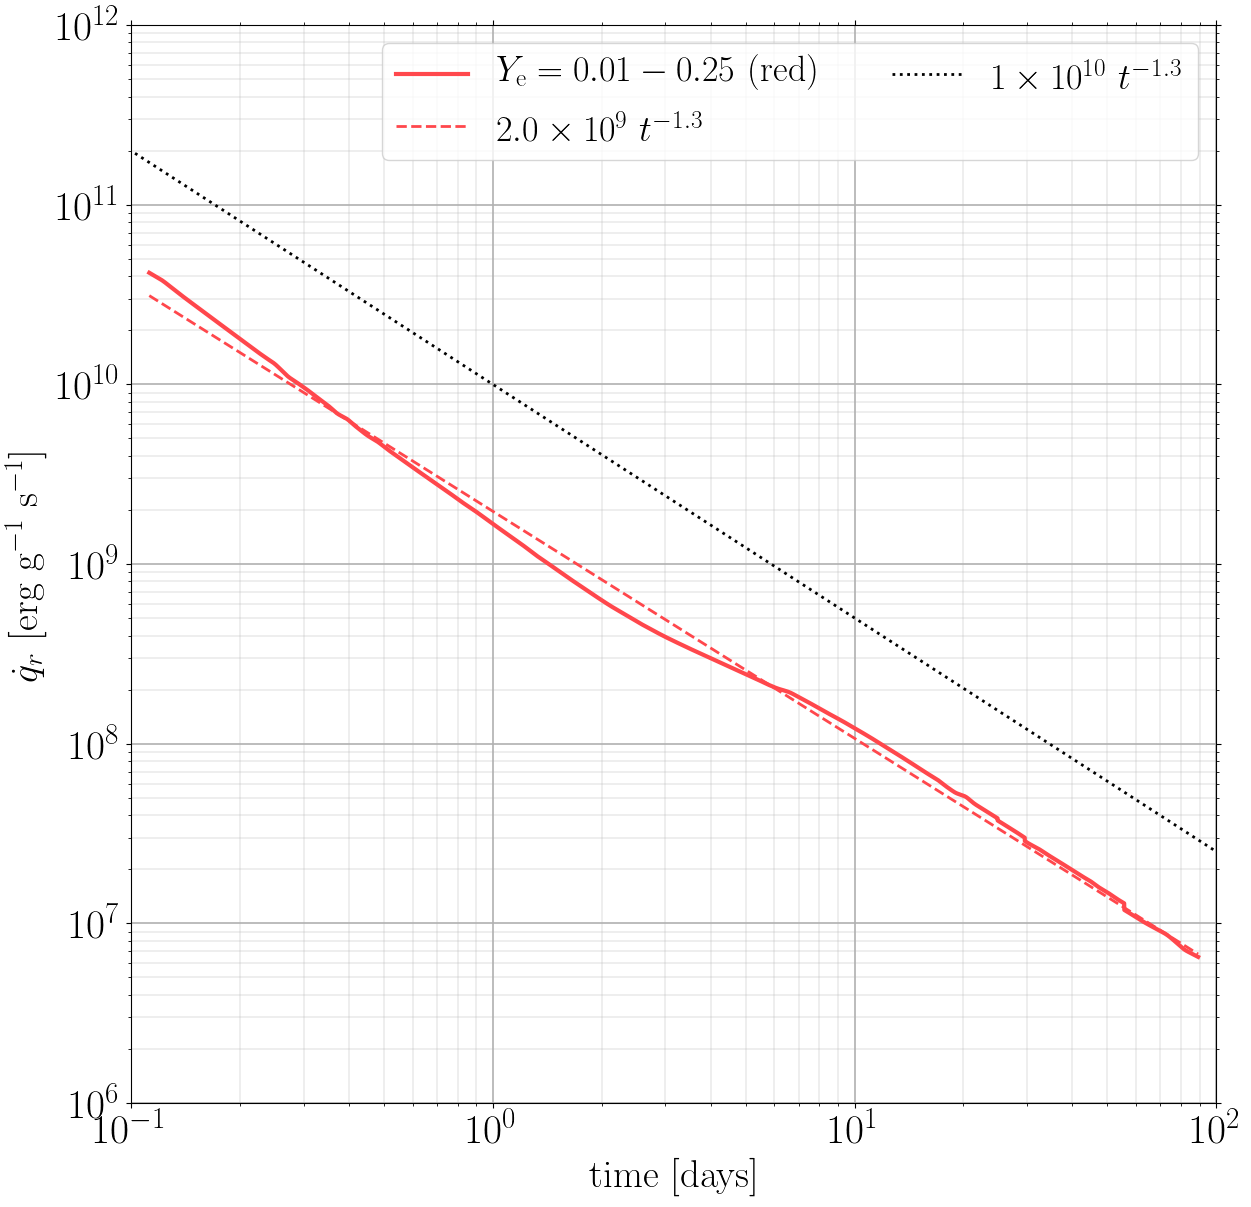
\includegraphics[scale=0.28]{figs/1_mFEa_Ye_RED.png}
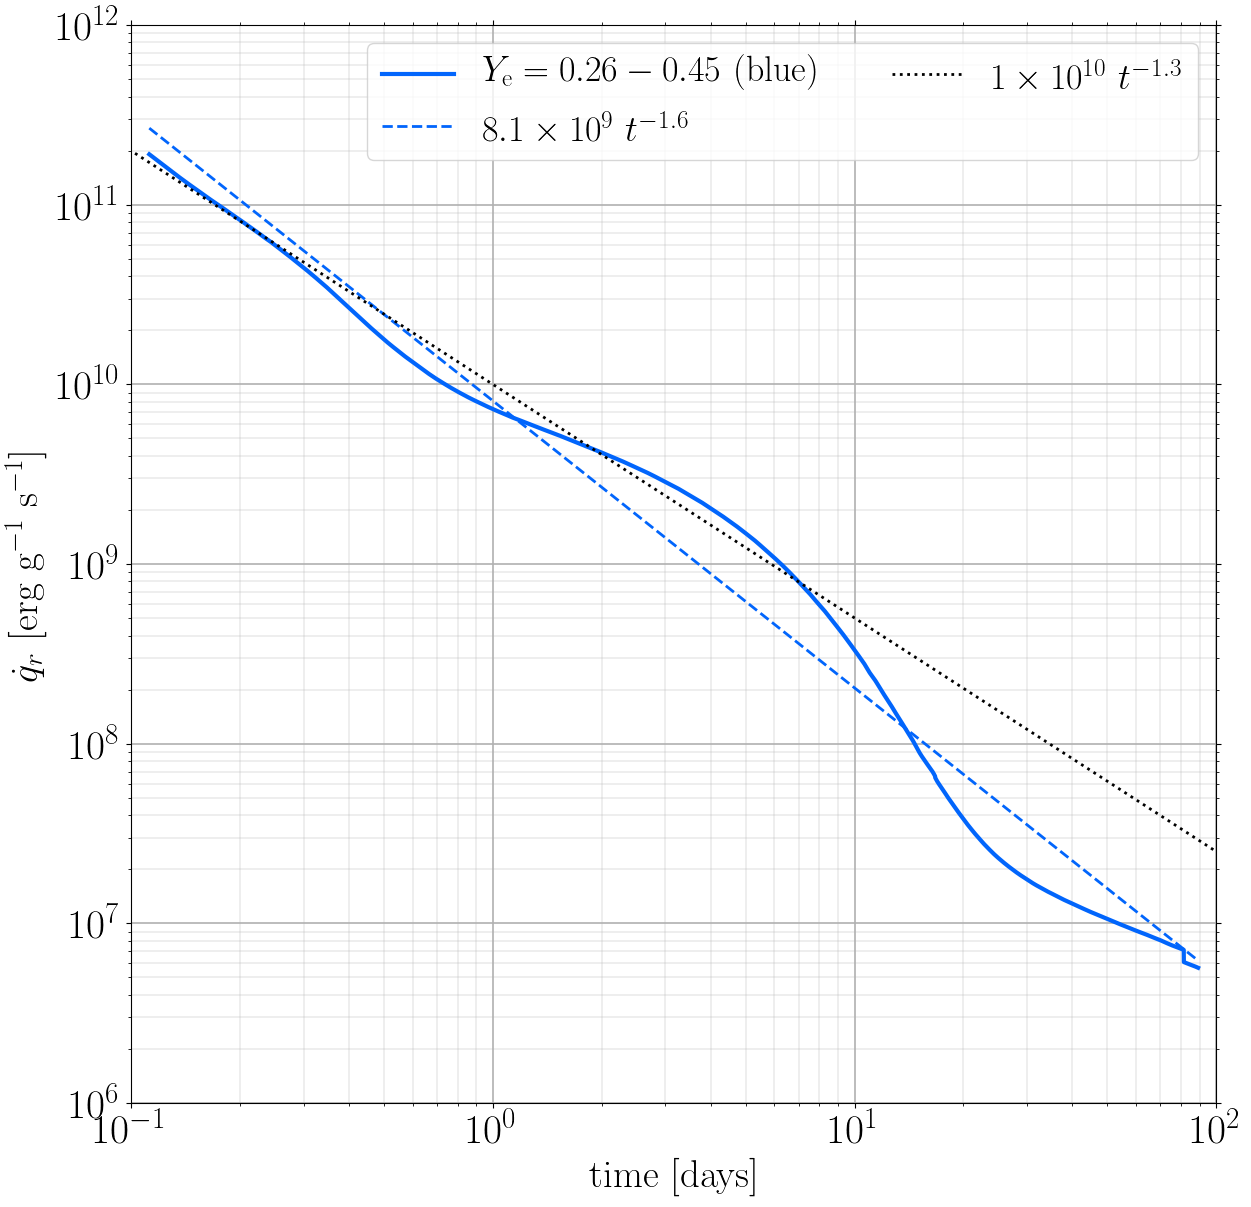
\includegraphics[scale=0.28]{figs/2_mFEa_Ye_BLUE.png}
}
\figcaption{\textbf{Heating rates contributed by a red and blue component of a kilonova, as computed in \cite{wanajo18}}. The left panel shows the contribution from a red component ($Y_\mathrm{e}=0.01 - 0.25$0, which is well-fit by a power law $\propto t^{-\alpha}$ with $\alpha=1.3$. The right panel shows the heating contribution from a blue component ($Y_\mathrm{e}=0.26 - 0.45$) and shows deviations from a power law. These deviations indicate that heating is dominated by a selection of radioactive isotopes rather than the ensemble of isotopes which is robustly produced in the red component. In both panels, the "empirical" power law given in Equation (\ref{eqn:qdot_plaw}) is shown for comparison.}
\label{fig:plaw_fits_W18}
\end{figure*}
% ============================

\end{document}